\documentclass{beamer}

\mode<presentation>
{
  \usetheme{CambridgeUS}
  \setbeamercovered{transparent}
}

\usepackage[english]{babel}
\usepackage[latin1]{inputenc}
\usepackage{times}
\usepackage[T1]{fontenc} 
% Or whatever. Note that the encoding and the font should match. If T1
% does not look nice, try deleting the line with the fontenc.
\usepackage{amsmath}

\newcommand{\linespace}{\vskip 0.25cm}

\definecolor{MyForestGreen}{rgb}{0,0.7,0} 
\newcommand{\tableemph}[1]{{#1}}
\newcommand{\tablewin}[1]{\tableemph{#1}}
\newcommand{\tablemid}[1]{\tableemph{#1}}
\newcommand{\tablelose}[1]{\tableemph{#1}}

\definecolor{MyLightGray}{rgb}{0.6,0.6,0.6}
\newcommand{\tabletie}[1]{\color{MyLightGray} {#1}}

% The text in square brackets is the short version of your title and will be used in the
% header/footer depending on your theme.
\title[Mobile Security]{Improving Mobile Security}

% Sub-titles are optional - uncomment and edit the next line if you want one.
% \subtitle{Why does sub-tree crossover work?} 

% The text in square brackets is the short version of your name(s) and will be used in the
% header/footer depending on your theme.
\author[Luthi]{Braden Luthi}

% The text in square brackets is the short version of your institution and will be used in the
% header/footer depending on your theme.
\institute[U of Minn, Morris]
{
  Division of Science and Mathematics \\
  University of Minnesota, Morris \\
  Morris, Minnesota, USA
}

% The text in square brackets is the short version of the date if you need that.
\date[April '14, ] % (optional)
{29 April 2014 }

% Delete this, if you do not want the table of contents to pop up at
% the beginning of each subsection:
\AtBeginSection[]
{
  \begin{frame}<beamer>
    \frametitle{Outline}
    \tableofcontents[currentsection, hideothersubsections]
  \end{frame}
}

\begin{document}

\begin{frame}
  \titlepage
\end{frame}

% For a 20-25 minute senior seminar talk you probably want something like:
% - Two or three major sections (other than the summary).
% - At *most* three subsections per section.
% - Talk about 30s to 2min per frame. So there should probably be between
%   15 and 30 frames, all told.

\section*{Overview}


\subsection*{Outline}

\begin{frame}
  \frametitle{Outline}
  \tableofcontents[hideallsubsections]
\end{frame}
\section{Background}
\subsection{Cryptography}

	\begin{frame}
	\frametitle{Cryptography}
	
		Cryptography or 'secret writing' is the study and practice of techniques for securing communications between two parties. \linebreak
		\begin{itemize}
			\item \textbf{plain-text}  Readable message to be sent during communications.
			\item \textbf{cipher-text} Unreadable form of the message
			\item \textbf{key} parameter for cryptographic algorithm or cipher		
			\item \textbf{cipher} method for transforming plain-text
			\begin{itemize}
				\item \textbf{Encrypt} transform plain-text to cipher-text
				\item \textbf{Decrypt} transform cipher-text back into plain-text
				
				
			\end{itemize}
	        		
			
			%--add toy cipher example--%
		\end{itemize}		 
	%basic introduction to cryptography and vocabulary
	
	\end{frame}
	\begin{frame}
	\frametitle{Cryptography}
		\begin{itemize}
			\item \textbf{Symmetric cryptography} 
			Both parties share a secret key for encryption and decryption
			\item \textbf{Asymmetric cryptography}
			Each individual has a public and a private key. Parties use the public keys for encryption and the private keys for decryption
		\end{itemize}
		%--add Asymmetric example--%
	
	\end{frame}

\subsection{GSM and UMTS}
	
		\begin{frame}
		\begin{itemize}
		\item Global System for Mobile Communications (GSM) is a 2G telecommunication standard developed in the early 90s by the European Telecommunications Institute. Has become one of the most widely used standards, reaching an 80\% market share at its height.
					
		
		\item Universal Telecommunications Standard (UMTS) is 3G telecommunication standard based on GSM by the Third Generation Partnership Project in the early 2000s.   
		\end{itemize}
		%--Mention interworking networks here--%
	\end{frame}

	
\section{GSM Weakness in UMTS}

	

	\begin{frame}
	\frametitle{Encryption in GSM and UTMS}
	\begin{itemize}
	
	
		\item GSM and UMTS both have secret keys that are shared between the mobile and the mobile's home network authentication center.
		
		\item GSM and UMTS both utilize the A5 family of encryption algorithms. 
		 \begin{itemize}
			\item A5/0 
			\item A5/1
			\item A5/2
			\item A5/3 
		\end{itemize}
		\end{itemize}
	\end{frame}
	
\subsection{Authentication}

%-----------GSM Authentication-----------------%
	% Talk Mention GSM weakness to Man in the middle Attack
\begin{frame}
% add hidden frames, introduce requests one at a time
  \frametitle{GSM Authentication}
  \begin{center}
  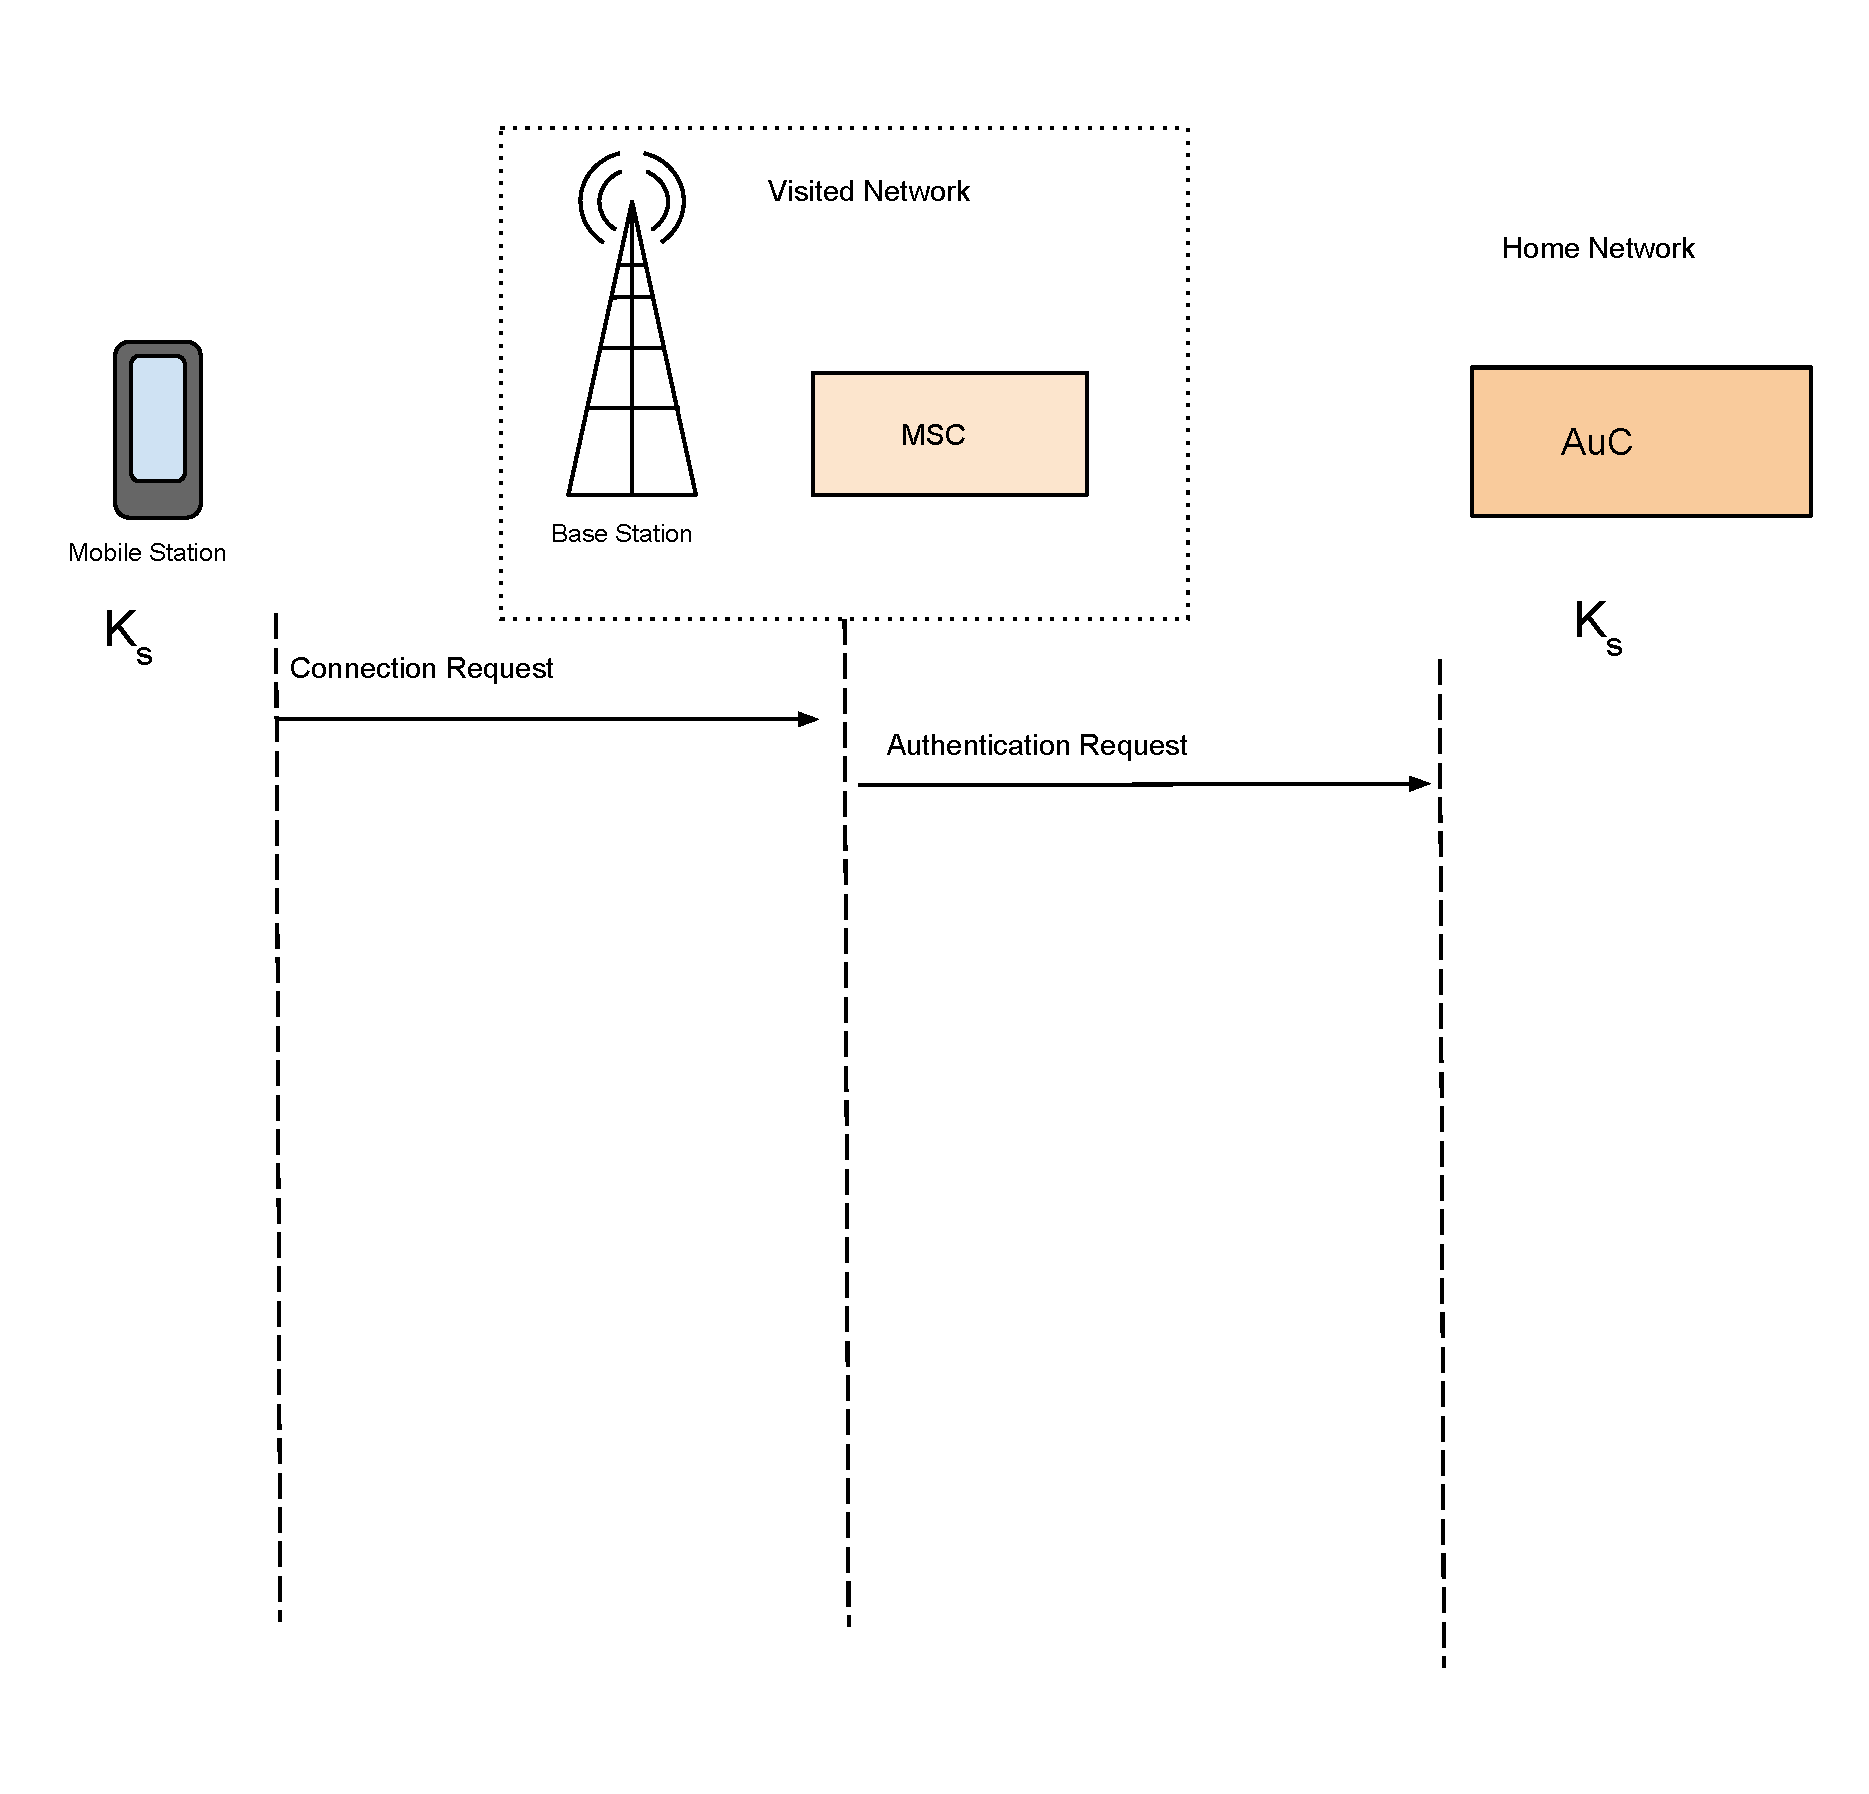
\includegraphics[width=.9\textwidth, height=.85\textheight]{Images/GSMAuthentication1.pdf}

  \end{center} 
\end{frame}
\begin{frame}
% add hidden frames, introduce requests one at a time
  \frametitle{GSM Authentication}
  \begin{center}
  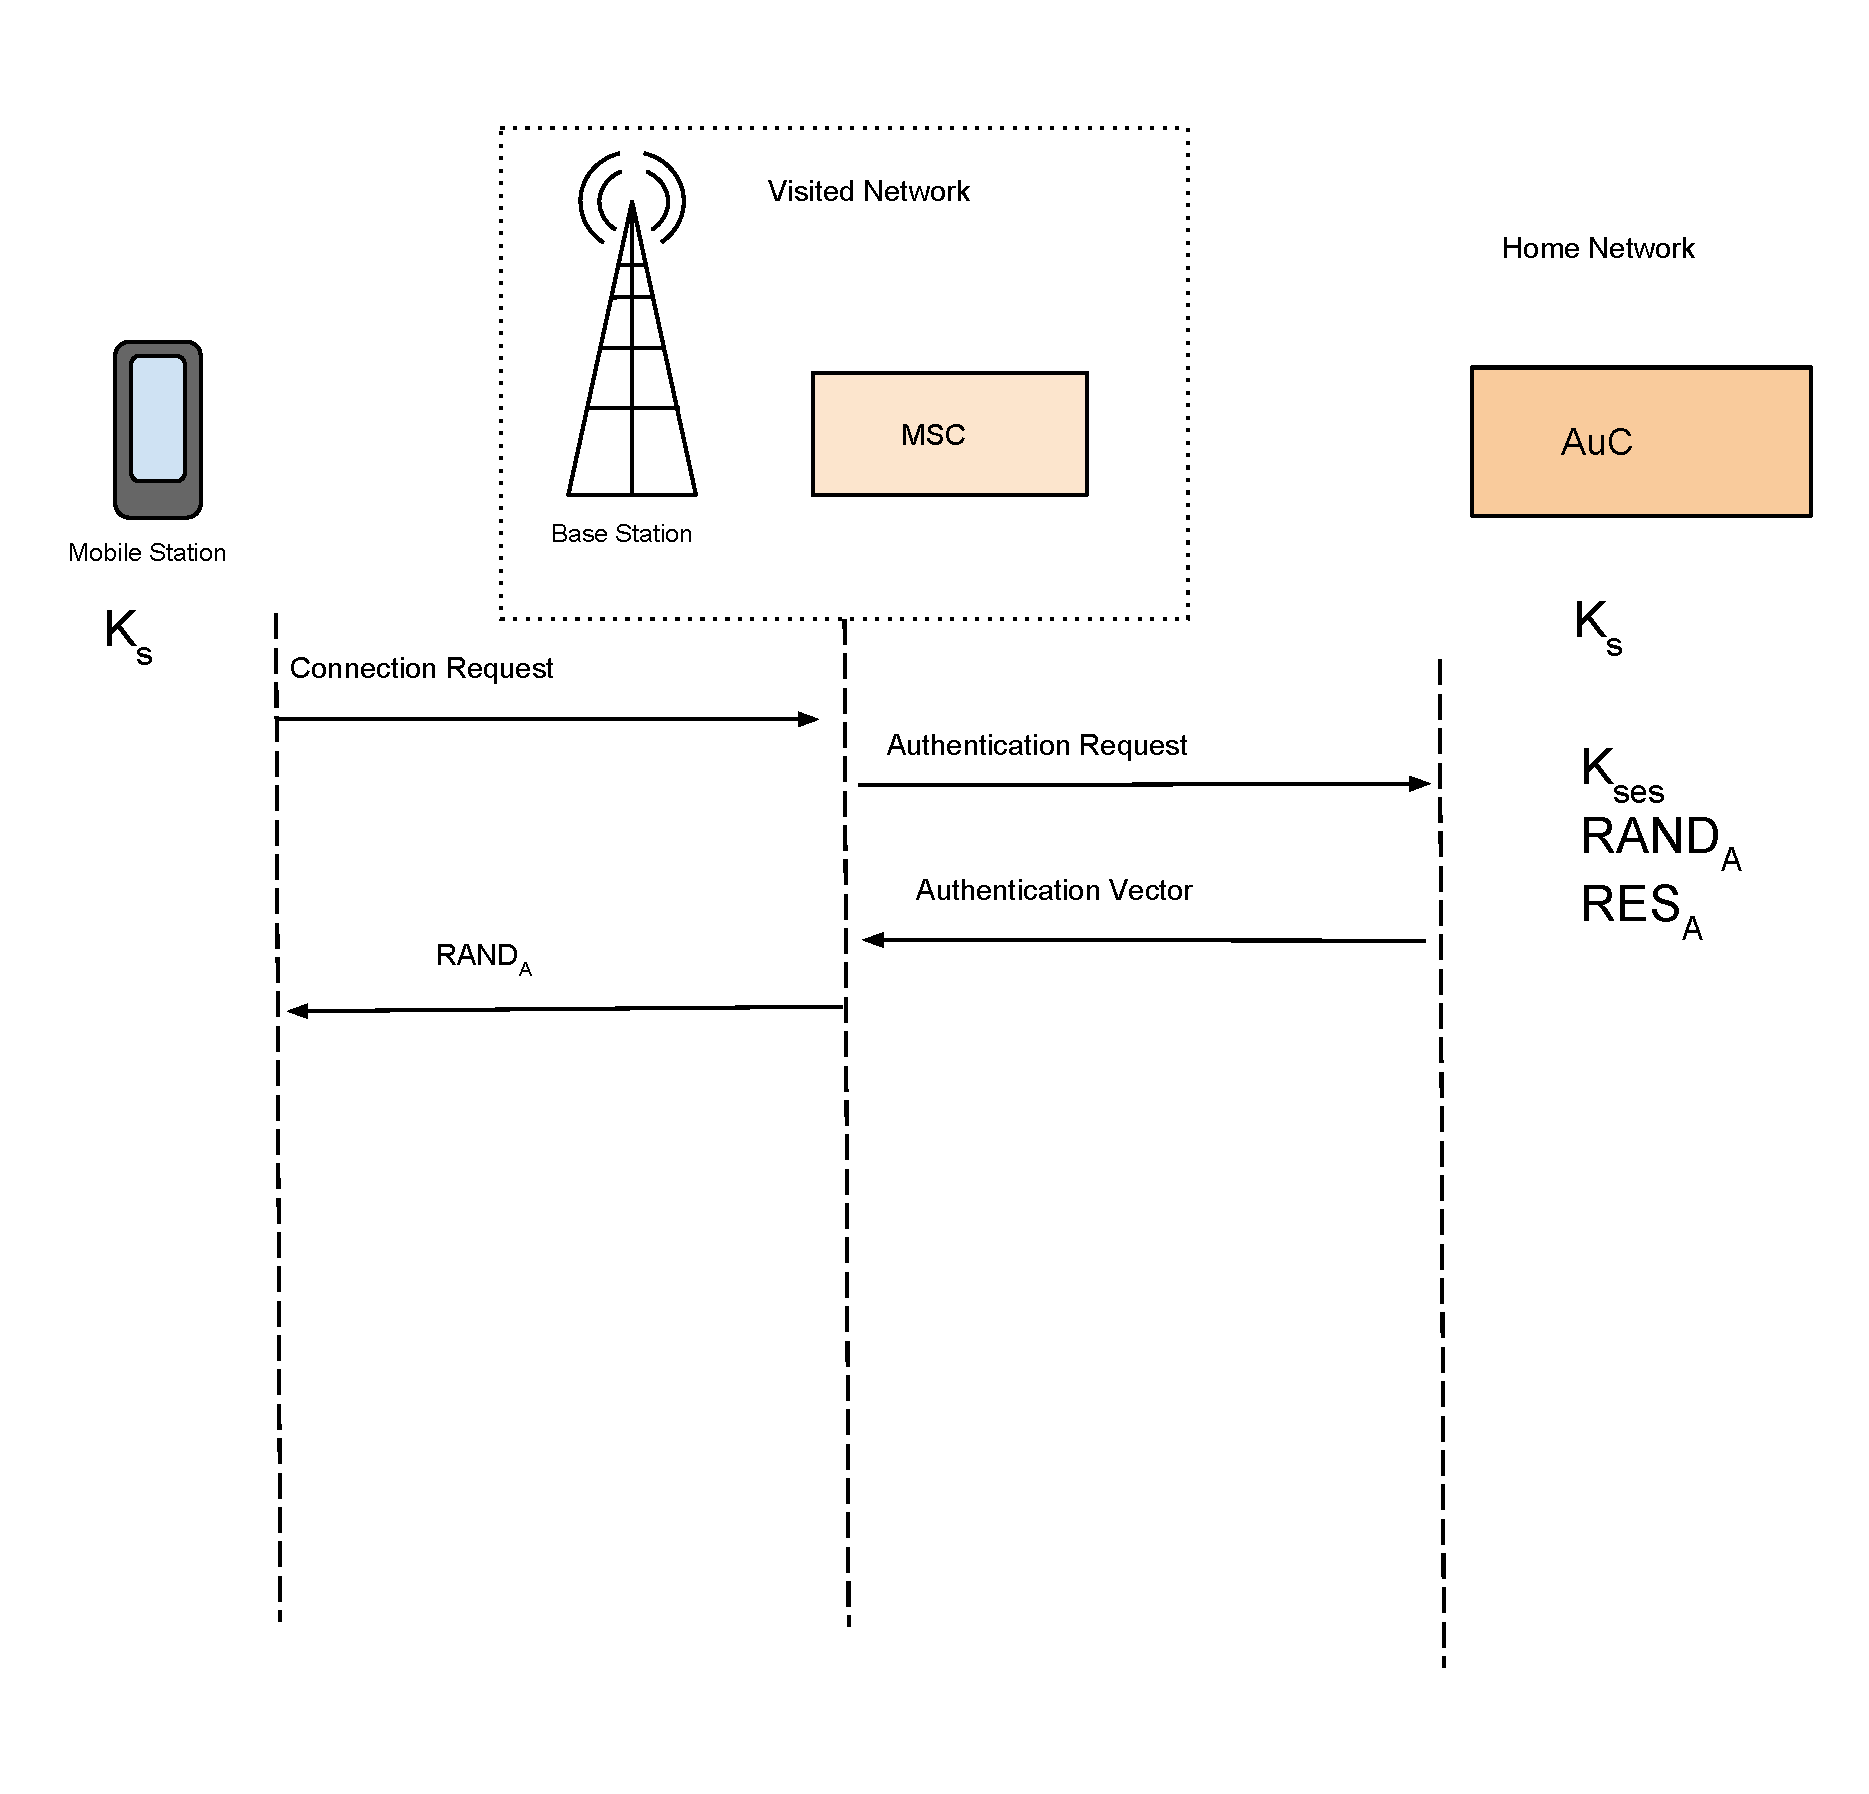
\includegraphics[width=.9\textwidth, height=.85\textheight]{Images/GSMAuthentication2.pdf}

  \end{center} 
\end{frame}
\begin{frame}
% add hidden frames, introduce requests one at a time
  \frametitle{GSM Authentication}
  \begin{center}
  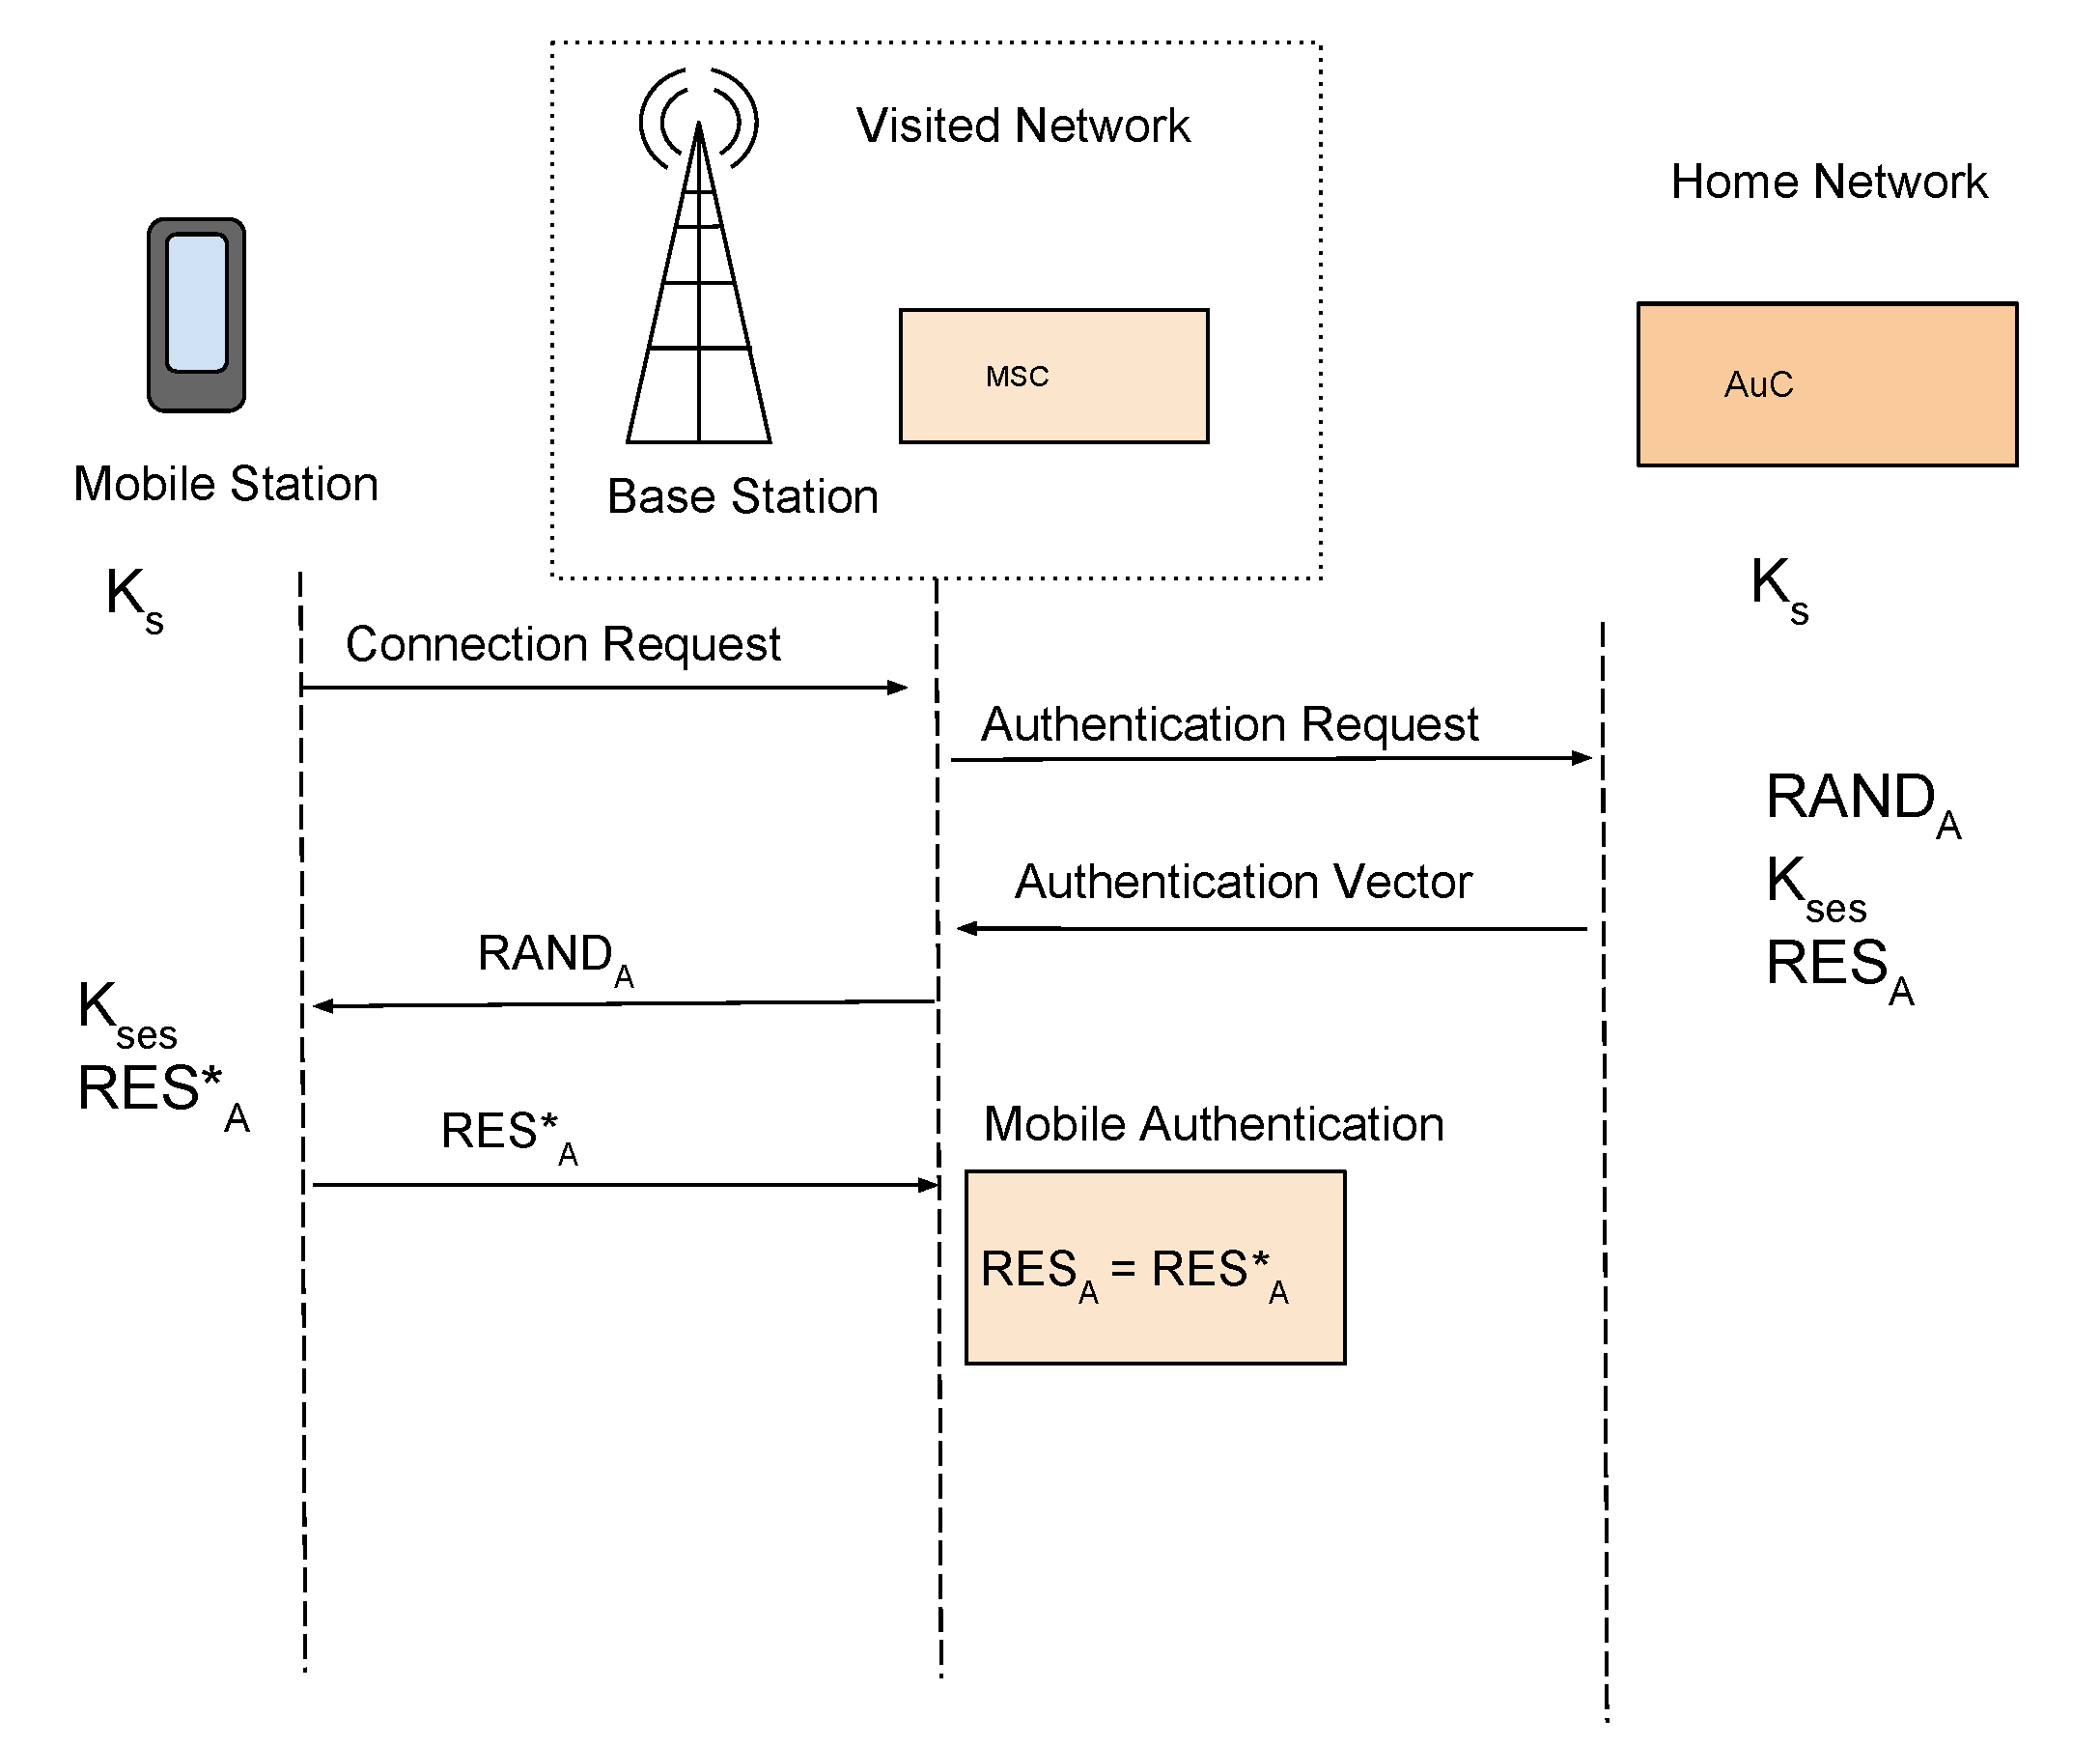
\includegraphics[width=.9\textwidth, height=.85\textheight]{Images/GSMAuthentication3.pdf}

  \end{center} 
\end{frame}
\begin{frame}
% add hidden frames, introduce requests one at a time
  \frametitle{GSM Authentication}
  \begin{center}
  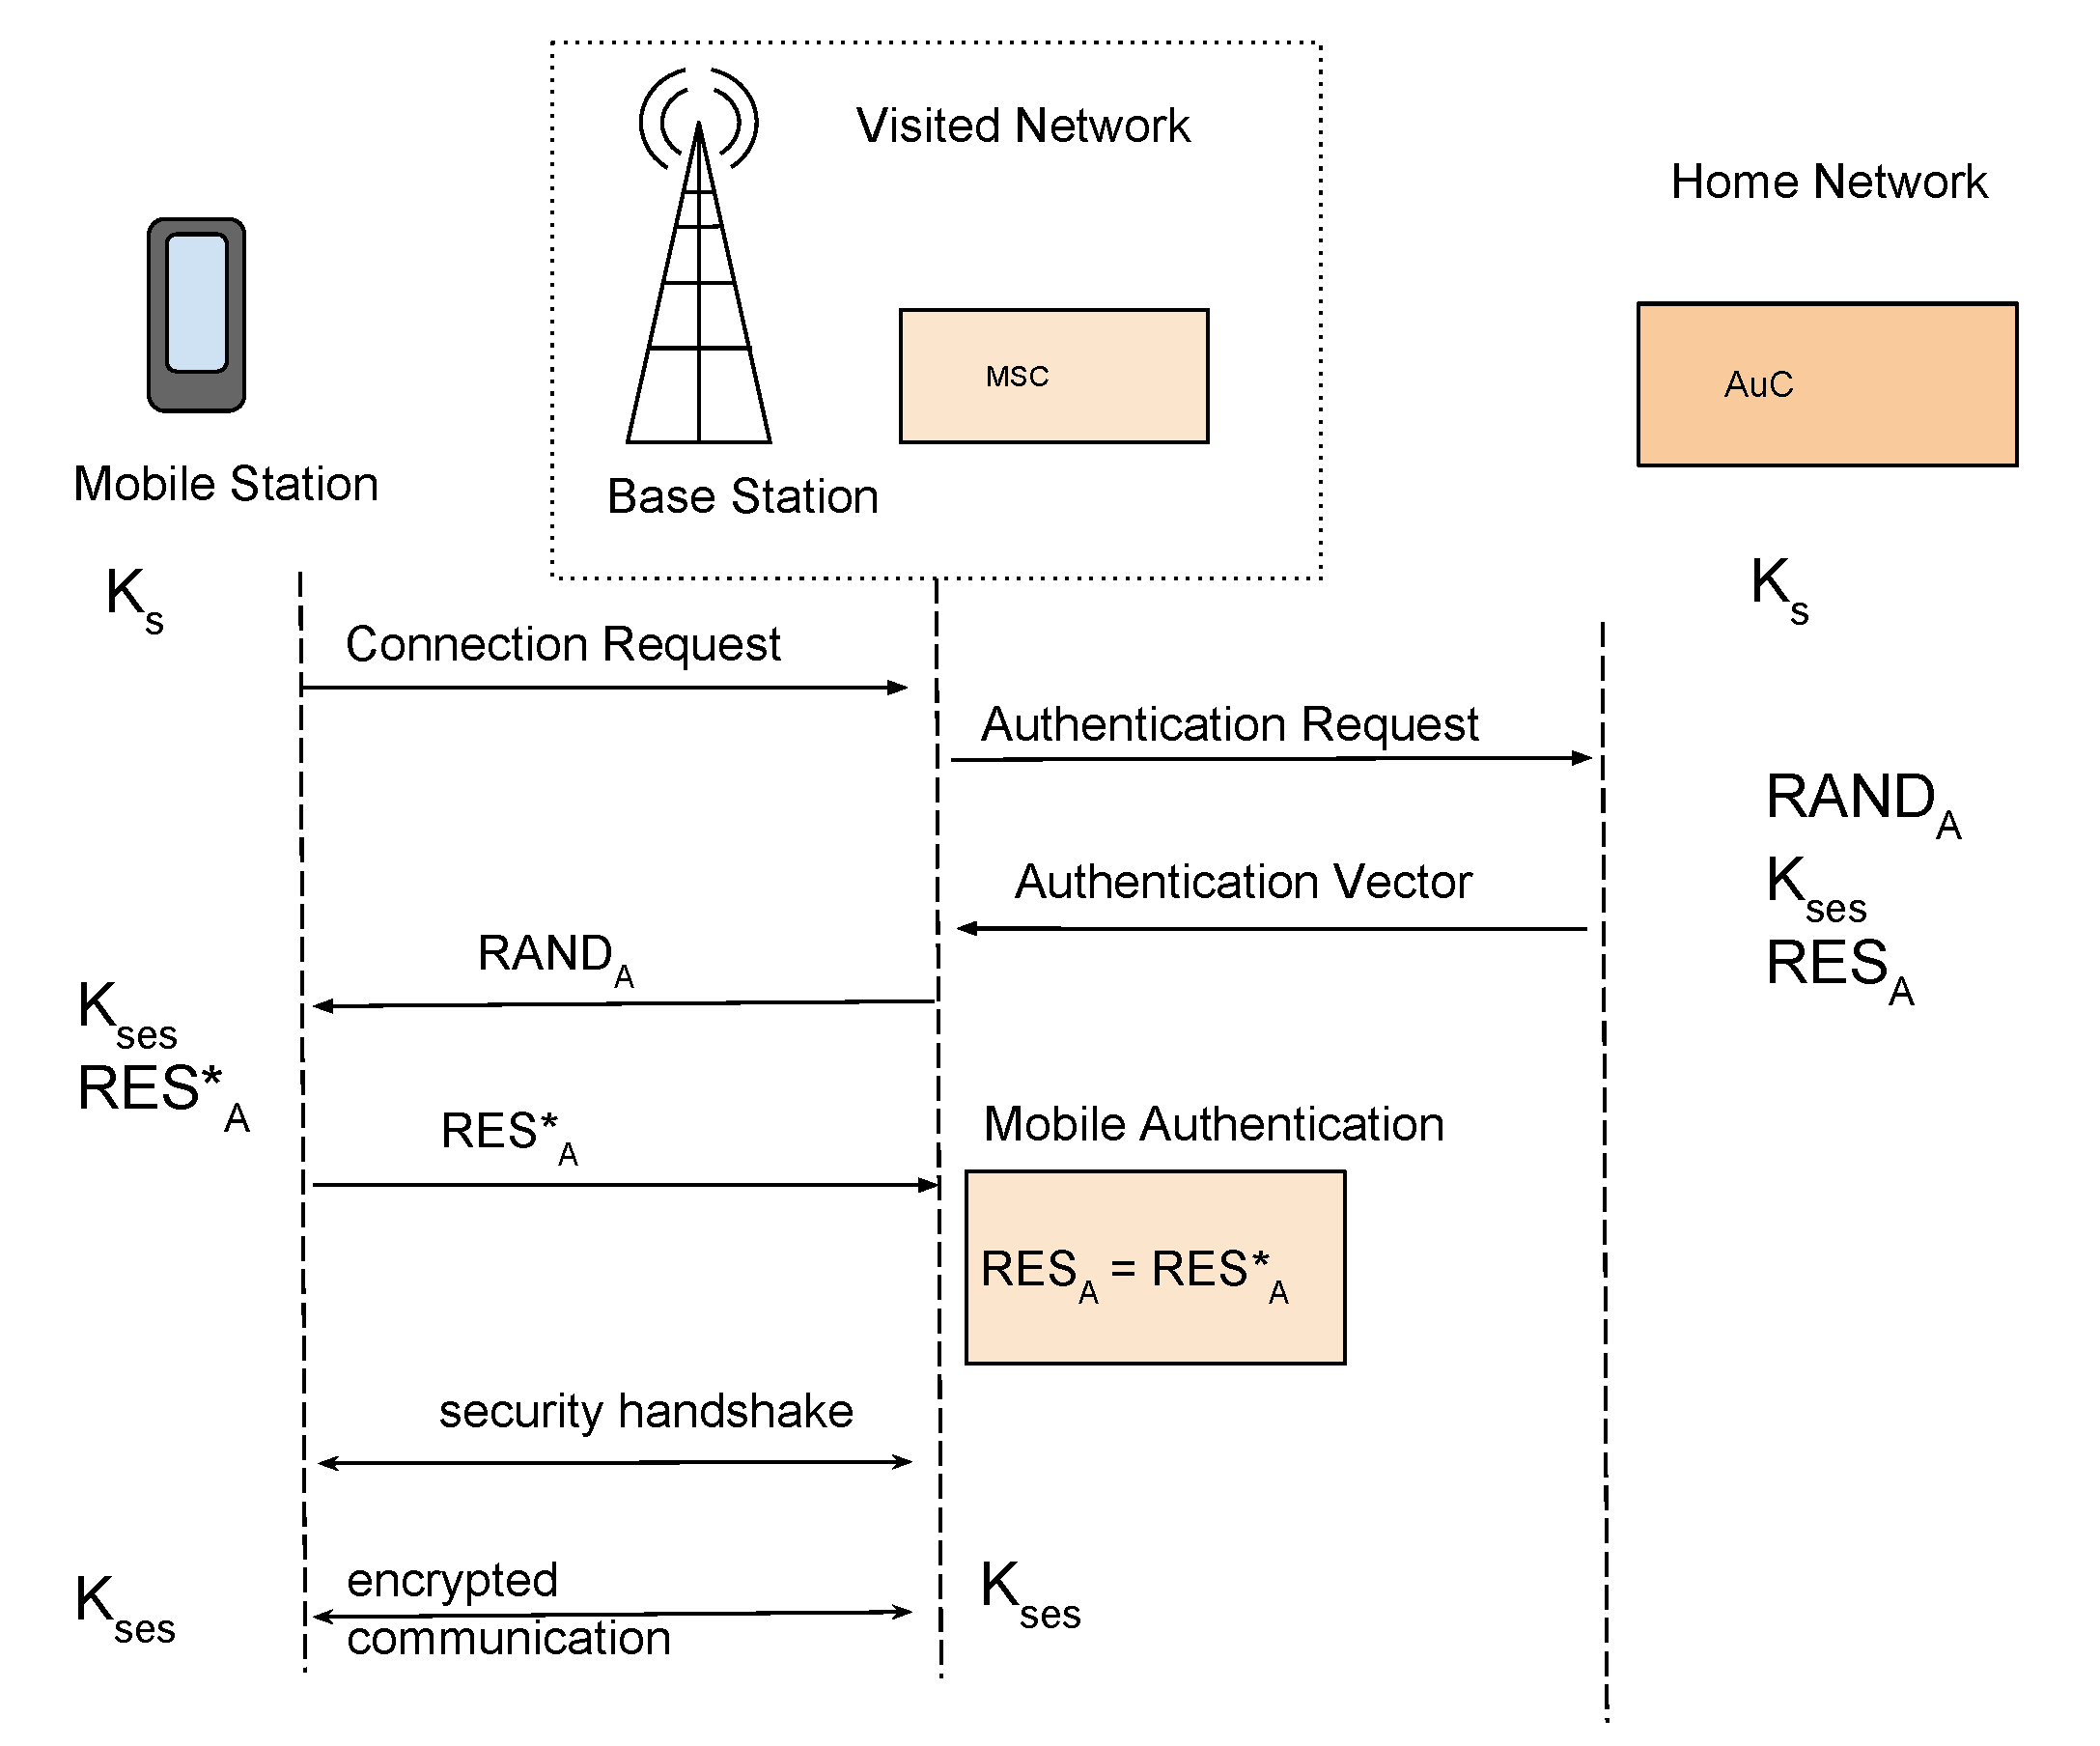
\includegraphics[width=.9\textwidth, height=.85\textheight]{Images/GSMAuthentication4.pdf}

  \end{center} 
\end{frame}

\subsection{Man-in-the-middle Attack}
\begin{frame}
		\frametitle{Man-in-the-middle Attack}
		\begin{columns}
		\begin{column}[T]{5cm}
		Man-in-the-middle attack is a type of attack in Cryptography where an attacker tricks participants into sending their communications through the attacker.   
		\end{column}
		\column{.5\textwidth}
		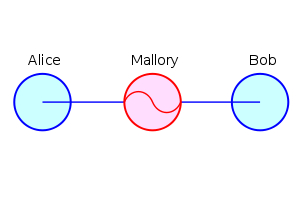
\includegraphics[scale=.45]{Images/MIM.jpg}
		\end{columns}
		\end{frame}
		
		\begin{frame}
	\frametitle{Man-in-the-middle Attack}
		TODO: add Example Diagram of Man-in-the-middle attack modeled after example in paper.	
\end{frame}
		% add man in the middle attack example		
%-----------UMTS Authentication-----------------%

\subsection{GSM and UMTS Inter-working Networks}
\begin{frame}
	\frametitle{Transitional Networks}
	TODO: bullet points?\\
		There are transitional periods between old and new technologies such as GSM and UMTS are required as old infrastructure and devices are replaced with the new. During these periods both old and new technologies will need to be able to successfully interact with one another.
		\\2011 survey where 2G devices had around 90\% population coverage where as 3G only had 45\%
\end{frame}

	\begin{frame}
	
	\frametitle{GSM and UMTS Inter-working network}
	
	
	In order for GSM and UMTS systems to work all UMTS systems must be capable of performing GSM communication. For encryption this means there needs to be ways of transforming 128 bit UMTS keys into the 64 bit GSM keys 
	
	
		\begin{equation}
			\label{C_3}
			\mathit{K_{ses} = c_{3}(I_{K},C_{ses}) = C_{ses1} \oplus 					C_{ses2}\oplus I_{K1} \oplus I_{K2}}
		\end{equation}
		\begin{equation} 
			\label{C_4}
			\mathit{C_{ses} = c_{4}(K_{ses}) = K_{ses} \| K_{ses}}
		\end{equation}
		\begin{equation}
			\label{C_5}
			\mathit{I_{K} = c_{5}(K_{ses}) = K_{ses1}\oplus K_{ses2}\|					K_{ses}\|K_{ses1}\oplus K_{ses2}}
		\end{equation}
	
\end{frame}	
		
\begin{frame}
	\frametitle{GSM Man-in-the-middle weakness in UMTS}
	% refer back to GSM authentication diagram ?
\end{frame}
\subsection{Solution}
\begin{frame}
\frametitle{Protecting UMTS from GSM Man-in-the-middle attack}
\end{frame}
\section{Application Security Threat}
	\subsection{Applications}
		\begin{frame}
		\frametitle{Applications (Apps)}
		\end{frame}
		\begin{frame}
		\frametitle{Application Permissions in Android}
		\end{frame}
		\begin{frame}
		\frametitle{Application Threat keyboard Key-logger}
		\end{frame}
	\subsection{Solution}
		\begin{frame}
		\frametitle{KBS Checker}
		\end{frame}
\section{Electromagnetic Radiation Leaking Key Information}
	\subsection{Side channel attack}
		\begin{frame}
		\frametitle{What is a Side channel attack?}
		\end{frame}
		\begin{frame}
		\frametitle{RSA Example}
		\end{frame}
	\subsection{Side channel through EM }
		\begin{frame}
		\frametitle{Ranged Side channel}
		\end{frame}
		
		\begin{frame}
		\frametitle{Findings}
		\end{frame}
		
		\begin{frame}
		\frametitle{Solution}
		\end{frame}
\section{Conclusion}
	\begin{frame}
		\frametitle{Conclusion}
		\end{frame}	
		
		\begin{frame}
		\frametitle{Questions}
			\begin{center}
			\Huge Questions?
			\end{center}
		\end{frame}	

\end{document}


